\documentclass[10pt, a4paper]{article}
%%%%%%%%%%%%%%%%%%%%%%%%%%%%%%%%%%%%%%%%%%%%%%%%%%
\title{\textbf{The Current State of Spatial Paritioning Trees: A Literature Review}}
\author{Patrick C. Shriwise}
\date{\today}
%\institute{Department of Engineering Physics, University of Wisconsin-Madison, 1500 Engineering Dr, Madison, WI 53706, shriwise\@wisc.edu}

%%%%% packages and defs
\usepackage{graphicx}
\graphicspath{{./images/}{../images/}{./}}
\usepackage[font={small,it}]{caption}
\usepackage{color}
\usepackage{hyperref}
\hypersetup{
    colorlinks=true, %set true if you want colored links
    linktoc=all,     %set to all if you want both sections and subsections linked
    linkcolor=black,  %choose some color if you want links to stand out
}

\begin{document}

\begin{center}
  \textbf{A Monte Carlo Oriented Ray Tracing Kernel} \\
  \bigskip
  by \\
  \bigskip
  Patrick C. Shriwise \\
  \bigskip 
  at the \\
  \bigskip
  UNIVERSITY OF WISCONSIN - MADISON \\
  \bigskip
  2016
\end{center}

\newpage
\tableofcontents 

\section{Abstract}

The value of CAD-Based Monte Carlo relies heavily on the ability to return geometric queries quickly and robustly via ray tracing. The Direct Accelerated Monte Carlo (DAGMC) toolkit currently provides a robust ray tracing algorithm\cite{thesis_smith_2010} given certain mesh requirements are met, but shortcomings of the underlying ray tracing kernel causes it to lag behind run times of a given Monte Carlo code using its native geometric analysis. Up to this point, we have relied on research in ray tracing mainly for the application of rendering or collision detection. Neither of these applications align exactly with the application of Monte Carlo ray tracing. Algorithms for collision detection involves moving geometry which isn’t yet a concern in the area of radiation transport. Algorithms for acceleration structures in rendering typically prioritize the time needed for the building of these structures causing them to be less than optimal, but results in an overall decreased time-to-render due to the balance of the build time with the number of ray queries needed to generate the desired graphics. In radiation transport, the number of ray queries needed to generate the desired result is much larger than the number needed for rendering. As more time is spent ray tracing, the build times of the underlying acceleration structures becomes less significant, thus the balance between time spent building these structures and the time using them for ray tracing must be reconsidered in this context. Its is hypothesized that in the case of the large, complex problems for which DAGMC is intended, that extra time spent optimizing the ray tracing acceleration structures via adaptation to certain mesh features and/or mesh refinement/alteration if necessary. This shift in priorities regarding the building process is important, but there are other improvements to be made as well. An area where the application of rendering and radiation transport align very well is in the query process after building of acceleration structures is complete. There are many advancements in ray tracing techniques which can be applied in order to provide further improvements to DAGMC’s performance. It is hoped that the combined effect of these improvements will bring DAGMC’s performance close to that of the native Monte Carlo codes it supports, thus alleviating the concern for additional computational time while maintaining the benefit of reduced human effort in radiation transport on complex geometric models.

\section{Introduction}

%% The purpose of this document is to outline the current state of the art in spatial partioning hierarchies for the purpose of improving performance in DagMC. It will take into account as much of the existing literature as possible. An analysis of the literature will also be conatined, identifying areas for improvement within the context of ray tracing for the specific application of Monte Carlo ray tracing.


The (DAGMC) toolkit \cite{dagmc_2009} robustly tracks particles through geometries represented by a surface mesh provided by the graphics faceting of the CAD engine in which the geometry is generated. Thanks to the make\_watertight algorithm\cite{make_watertight_smith_2010} DAGMC can robustly track particles through highly complex geometries by providing the necessary geometric information to underlying Monte Carlo physics codes via the ray tracing kernel in the Mesh Oriented dAtaBase (MOAB)\cite{moab}.

Naturally following the ability to do these robust calculations on already complex models, increasingly detailed models are becoming of interest. As detail increases, the performace of DAGMC lags more and more in comparison to the native versions of the various Monte Carlo codes it supports. It has long been known that this performance issue is due to the time it takes to return geometric information to Monte Carlo packages from the ray tracing kernel. Recent profiling of the DAGMC code supports this knowledge. This work has shown that in complex models ~85\% of the run time is spent in the ray tracing kernel. As this area seems to be the main bottleneck, this work will focus on optimizing this area in DAGMC.

The purpose of most applications involving ray tracing is rendering. Techiques used in rendering for accelerating ray tracing queries have proved very useful in the area of Monte Carlo analysis. However, these techniques have largely been applied without modification or adaptation for the purposes of ray tracing in Monte Carlo. Several fundamental differences exist between the two applications. Exploration of how ray tracing kernels inteded for use in Monte Carlo codes can be modified to the benefit of performance will be explored in this work.

* we fire more rays, damnit! affects time to solution
* also, SIMD could be a big win (espeically for history-based threading)
* we know what volume we're in

\section{Ray Tracing's Role in Monte Carlo}

Ray tracing is most commonly used to generate 2D images by simulating light ray interactions with virtual 3D objects in a process known as rendering. These light rays (photons) are typically cast from the perspective of the image to be generated, and pixel colors are determined by the reflections, refractions, etc. of the photons on their course to the light source (if they reach it at all). This process is analagous to Monte Carlo analysis. Particles are born at the source and go through a series of interactions with 3D objects until they reach an area of interest, or detector, at which point data related to the particle is collected and stored. In both cases, when particles obtain new orientations from their interactions in this virtual 3D space, it is necessary to understand what object this particle will interact with next if it continues on its current trajectory. As such, the problem of ray tracing in either application can be abstracted to a spatial search of a virtual 3D object for the next interaction location given a particle loaction and trajectory. 

In realistic renderings, it is sometimes possible that light rays may scatter before reaching the next object on their path and in Monte Carlo simulations this is the more probable case. In order to determine if this will occur before reaching the next object, the distance to interaction (scattering or otherwise) must be compared to the distance to the next object. In analytic geometric representations this is a straightforward task, but as the complexity of 3D objects increase, the cost of ray-object intersections becomes very computationally expensive. Mesh/CAD-based models, in which the surfaces of objects are discretized into sets of geometric primitives (usually triangles), face the challenge of then finding the correct primitive for which the ray intersects (if it intersects one at all). For the highly complex models, a linear search of the primitives is out of the question in terms of how long these intersections would take to find. As a result, extensive research has been done in the area of acceleration data structures for ray tracing which section the problem space in order to establish a binary tree-like search over the geometric primitives of the model.

\section{Spatial Partitioning Schemes}

Spatial partioning structures are designed to rapidly narrow the search for a location in virtual space given a location and orientation. This is accomplished by sectioning the space using a partitioning construct. The paritions are determined by a division heuristic which establishes the partitions given a set of primitives. After partitioning, the primitives are then associated with the partition which contains them. This process is recursively repeated until leaf conditions are met. Leaf conditions determine when the partioning process will stop. This can be based on the remaining number of primitives, the current size of the partition, etc. The end result is a hierarchy which can be used to terverse the problem space efficiently for ray intersections or closest intersection queries. 

The above describes a top-down approach to construction of these data structures, however, bottom-up construction does exist in which leaf partitions are created in accordance leaf conditions. These partitions are then joined recursively to create progressively larger partitions until all the primitives of interest are in a single partition. While most hierarchies are binary, having two children per interior node, the number of partitions per level in the hierarchy can change to better fit division heuristics or partitioning constructs. A variety of well established spatial partitioniong hierarchies exist with different structure hierarchies, partitioning constructs, division heuristics, and leaf conditions.

%% The tree structure refers almost entirely to the number of children each non-leaf node in the tree should have. The majority of spatial trees are binary trees (two children), but other structures do exist such as quad trees (four children) and oct trees (eight children). The partitioning construct refers to the mechanism by which you are creating partitions out of space. There is a large variety of these which are chosen based on a couple of counteracting criterion 1) number of operations required for an intersection check and 2) their ability to effectively eliminate subsets of the problem space from a given query.
 
\subsection{Bounding Volume Hierarchy (BVH)}

The initial concept of using the bounding volume partitioning construct as a pre-check for ray-intersection with objects was introduced by Weghorst in 1984 \cite{Weghorst:1984:ICM}. Weghorst explored the possibility of using spheres and rectangular parallell pipeds (boxes) to contain geometric objects. This work also went so far as to create a hierarchy of those object-based bounding volumes, noting the importance of hierarchicaly joining bounding volumes which are near each other in space so as not to have parent volumes containing large amounts of empty space between the objects to be joined.

Over time it was found that complex geometric objects become difficult to render as the analytic calculation of ray intersections became more costly. As a result, representations of geometric objects were then discretized for rendering purposes. The ray interactions with these more simple geometric primitives (usually triangles) are much less costly to compute in comparison to the previous analytic representation. Given that the geometric object can be discretized accurately, this also allows for the rendering of arbitrarily complex geometric objects without the need for continuous development of efficient analytic intersection techniques for all classes of complex parametric surfaces. Hierarchies of bounding volumes could then be created on subsets of the primitives, making for deepter and even more effective accelerations of ray tracing.

One difficulty bounding volume hierarchies face is the overlapping bounding volumes. Overlapping sibling volumes can cause additional box intersection checks in the same way that losely fitting boxes can. If a ray enters a region of overlapping sibling volumes, this causes the children of both boxes to be checked despite the fact that the ray will eventually only intersect with the desendants of one box or the other. Overlaps will almost always occur as boxes are required to contain discrete elements for robustness, not just a section of the virtual space. This inefficiency can be exacerbated by the types of triangles or regions of the discretized geometry the data structures are being formed around.


\subsubsection{Axis Aligned Bounding Box Hierarchies}

Axis aligned bounding boxes are boxes whose faces are parallel to the global planes of the problem space as defined by the global axes of the problem. In practice, tightly fitting axis aligned boxes are straightforward to construct given a set of points to contain, and overlaps between the children of a parent box are minimal. The overlaps found in axis aligned bounding boxes are typically limited to the size of perhaps one or two geometric primitives. Axis aligned boxes are commonly used in BVH's for their simplicity of implementation and fast ray intersection check algorithms.

In addition to the previously mentioned contributions of Weghosrt above, another important conclusion was made regarding the types of boundng volumes used to construct these hierarchies. In his exploration of sphere and box bounding volumes it was found that while spherical bounding volumes are less compuationally expensive to check for ray intersections than bounding boxes, the latter generally provide a tighter fit to the objects they contain. This tighter fitting is important as it decreases the chance of wasted intersection checks. This affect was reflected in the results of Weghorts's work strongly enough to show that bounding boxes were more effective in accelerating the ray intersection process than bounding spheres. 


\subsubsection{Oriented Bounding Box Hierarchies}

Unlike axis aligned bounding boxes, the faces of oriented bounding boxes are allowed take any orientation whey like to enclose their set of primitives as tightly as possible. There are several existing methods for determining the orientation of a box for best fit to a set of primitives.\cite{gottschalk1996obbtree} As a result, oriented bounding boxes are very good for avoiding erroneous ray-box intersections that would otherwise occur for an axis aligned box, and they more quickly conform to the full set of enclosed primitives as the boxes are subdivided. This conformity indicates that oriented bounding box hierarchies will have fewer levels making the worst case number of intersection tests lower than for an axis aligned box hierachy on average.

One disadvantage of oriented boxes is the intersection check requires an extra step in transformation of the ray to the oriented axes of the box in question. The information needed for this basis transformation of the ray must be constructed and applied to the ray before the box intersection can continue as it would for an axis aligned box. So while the oriented box hierarchy may have fewer intersection checks to do for a given ray query than an axis aligned box, they intersection checks do take some extra time.

An additional complication of oriented bounding boxes is the potential for large overlaps in the child boxes of a parent box. 

As a result of this tight fit to primitives, bounding volume hierarchies are also used in the area of object interference detection. The same concept as ray tracing is used to do a pre-check of several box-to-box intersections before committing to a more computationally expensive intersection check on the geometric objects themselves.

Oriented bounding boxes have been found to be extremely effective in 


\subsection{Splitting Schemes}

Bounding Volume Heirarchies provide a means of recursively narrowing the focus of the ray query to more promising candidates for intersection. This is a natural divide-and-conquer approach for examining a set of primitives for the closest intersection. Spatial subdivision takes a different approach. \cite{Intro2RT} While it is still a divide-and-conquer approach to the problem, the focus is generalized to the problem space instead of on the object themselves. Beginning with the entire model, one partitions the volume bounding the primitives into pieces recursively, creating smaller partitions in each level of the tree until a subset of primitives is left bounded at the leaf node of the hierarchy. This method can arguably be viewed as a top-down approach to bounding volumes but with an emphasis on division of space rather than division of objects.


Many data structures have been created using this philosophy. Some methods use grids built from voxels to discretize space, while others use different constructs like hyperplanes. Uniforn and non-uniform grid methods both track which primitives intersect a given voxel and as a ray passes through the grid, only primitives within the current voxel (if any) are checked for intersection. Methods of recent interest divide space recursively using a hierarchy in the same way BVH's do, but using voxels or hyperplanes focused on dividing problem space rather than object bounding volumes.

% INCLUDE A GRAPH-BASED COMPARISON OF DIFFERENT HIERARCHIES HERE %

\subsubsection{KD-Trees}

The KD-Tree or multidimensional binary search tree was originally developed as a method for querying records in databases and has since found use in other applications including speech recognition, global information systems, and ray tracing. \cite{Bentley1975} KD-Trees operate by recursively dividing the dimensions of the problem set. Initally the entirety of a problem dimension is divided in half (if one is using median splitting). The resulting subsets of the dimension are labeled as children of the initial set. The two resultant sets are the partitioned as well, but in a different dimension than the original partition. This process is then repeated until the leaf conditions of the hierarchy are met. Entities are listed as contained by a partition only if they are contained by all parents of the partition as well, meaning that all entities lie within some subset in each dimension of the problem.

This process is easily applied to the virtual 3D space of CAD models for ray intersection queries. The problem space is divided evenly in the x dimension. The two child partitions are then divided along the y axis and the resulting children of this division are subdivided along the z axis. Divisions are typically done s.t. the space of the current candidate is separated in half, however it is possible that by doing this primitive entities are divided by the hyperplane as well. There two ways that this is typically handled. The first is to simply reference any primitives in both of the subdivisions. This has the effect of creating a small overlap between the partitions, but requires no changes to the original model. The other solution is to divide the primitive entities in two using the division plane. While in terms of data structure traversal, this solution requires alterations to the model which may be undesirable under certain conditions and violates the description of the KD-Tree as a query acceleration structure.

KD-Treees work very well for nearest neighbor searches in which the query

%Talk about subdivision methods here

%% 2-D Example from Bentley1975 here %%


\subsubsection{Bounding Interval Hierarchy}

The bounding interval hierarchy is an extension of the KD-Tree in which two planes are used to define an interval of one of the problem dimensions as a node in the hierarchy rather than dividing the dimension into two parts. While the intersection check for an interval is twice as long as a plane's intersection check, the interval excludes more of the problem space for negative intersection checks than a plane can. The interval partioning construct also allows for different tree designs as each dimension can be broken up into an arbitrary number of intervals. Bounding intervals face the same problem that KD-Trees face with planar partitions intersecting primitive entities. The option to split primitive entities along the intersecting planes still exists in this scenario and comes with the same consequences as before. Sharing entity references can actually cause overlaps on either side of the interval making this problem somewhat worse in that case.

%% Interval Overlap Figure Here %%

\subsubsection{Octrees}

Octrees are a recursive form of the grid-based methods mentioned above. In this partitioning scheme, cubic voxels are used to partition the problem space into the 8 quadrants defined by the axes of the parent voxel. These 8 voxels are then labeled as children of the original voxel. This process is repeated recursively until leaf conditions are met for the voxel. This typically means that the voxel references a set number of primitives.

Octrees consume a large amount of memory relative to the other data structures in this section and  it is often possible that voxels may be completely devoid of underlying entities. One advantage of octrees is the cubis nature of the partitioning voxels. The value of a voxel (or bounding volume for that matter) lies in its ability to remove candidate space from the query, yet this voxel can only be effective in this way if rays actually strike the voxel. The result is that a voxel's effectiveness is described by the ratio of its probability of an intersection check to the space it will exclude from the query search or its volume. In a problem with a uniform ray distribution, the probablity of a ray to intersect a given voxel is described by its surface area. Thus cubic voxels have the most favorable ratio possible.

\section{Ray Coherence in Radiation Transport}

Ray coherence refers to the likelyhood that a primary ray will follow roughly the same path through the scene or model if fired multiple times. This is generally true in ray tracing processes oriented toward rendering due to the nature of the physics being modeled in reflection/refraction of visible light interacting with object surfaces in a given scene. This ray coherence can be exploited by cacheing the traversal path of rays from a given pixel location and direction. This gives subsequent rays fired from that location with similar directions a short-scut in their traversal with modifications to the traversal path as needed to determine their proper object/primitive intersection. Rays from the same origin and similar direction are grouped together and traverse kernel's acceleration structure. If their path becomes unique, the ray will then split off to coplete its own unique traversal, but this saves time in repeated operations for multiple rays in many or most levels of the hierarchy traversal.

In the application of radiation transport, however, the properties of the underlying physics being modeled does not result in ray coherence. Particles in radiation transport travel far beyond the surface of an object and with a much wider range of possible interaction locations and resulting directions compared to the modeling of visible light. As a result, these methods could only be applied to special situations in which the ray origins will be known such as radiation sources. For the general case, however, it is suspected that the majority of ray queries for a given set of particle histories are not attributed to the initial particle path, but due to subsequent interactions in the model as well as the queries required to resolve the emission of secondary radition. Thus such methods are likely not worth applying in this case.

\section{Ray Generalization in Radiation Transport}



\section{Partioning Methods and Leaf Conditions}

This section will go over several of the partitioning hueristics and leaf conditions involved in creating these hierarchies.

\subsection{Median Splitting}

This method splits the current partition in half for a given dimension. In the case of bounding boxes this is typically done by splitting using the axis (oriented or axis-aligned) with the largest extent to matain bounding boxes which are as cubic as possible for reasons described in the section above on octrees.

\subsection{Median Snap Splitting}

\subsection{Subdivision Sample Splitting}

This methos is similar to the median splitting method, but samples serveral candidate locations along the dimension to be divided. This can provide for better splitting over the entities contained by the parent node. The idea here is that even space is being split evenly the entities may not be, resulting is unbalanced trees with more bounding volumes than necessary for good taversal performance. This conecpt is typically a concern of bounding volume hierarchies as opposed to KDTrees or Bounding Interval Hierarchies. 


\subsection{Vertex Median}

\subsection{Vertex Sample}

\subsection{Surface Area Heuristic}


\section{High Valence Vertex Study}

One of the known bottlenecks of DAGMC is ray tracing performance degredation in regions with high-valence vertices. High valence vertices are defined as those connected to an unusally high number of triangle entities. This region of the mesh usually takes on a fan-like shape as seen in the figure below. These regions typically occur in regions where a planar surface is bounded by a circular curve, which is quite common in the faceting scheme used to produce DAGMC meshes. This faceting scheme (which comes from ACIS libraries underlying the CUBIT/Trelis graphics engine) is designed to produce the smallest number of triangles possible to represent the model within the representation tolerance specified in the surface mesh generation preprocessing step (dagmc\_preproc). Generally fewer triangles are better as even the ideal ray tracing acceleration structure queries for a given mesh scale as $O(log(N))$. However, even with fewer triangles undesirable configurations of mesh can impede performance as we will see here.

\begin{figure}
  \centering
    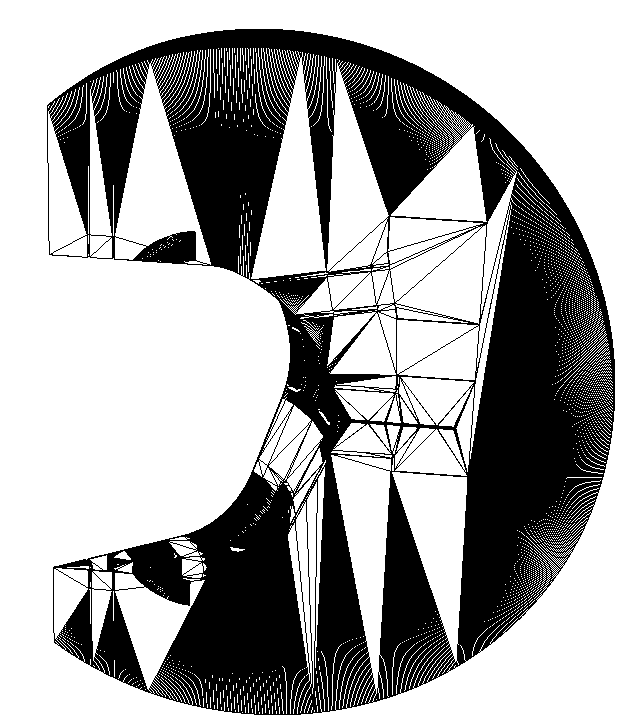
\includegraphics[scale=0.2]{iter_sideon.png}
    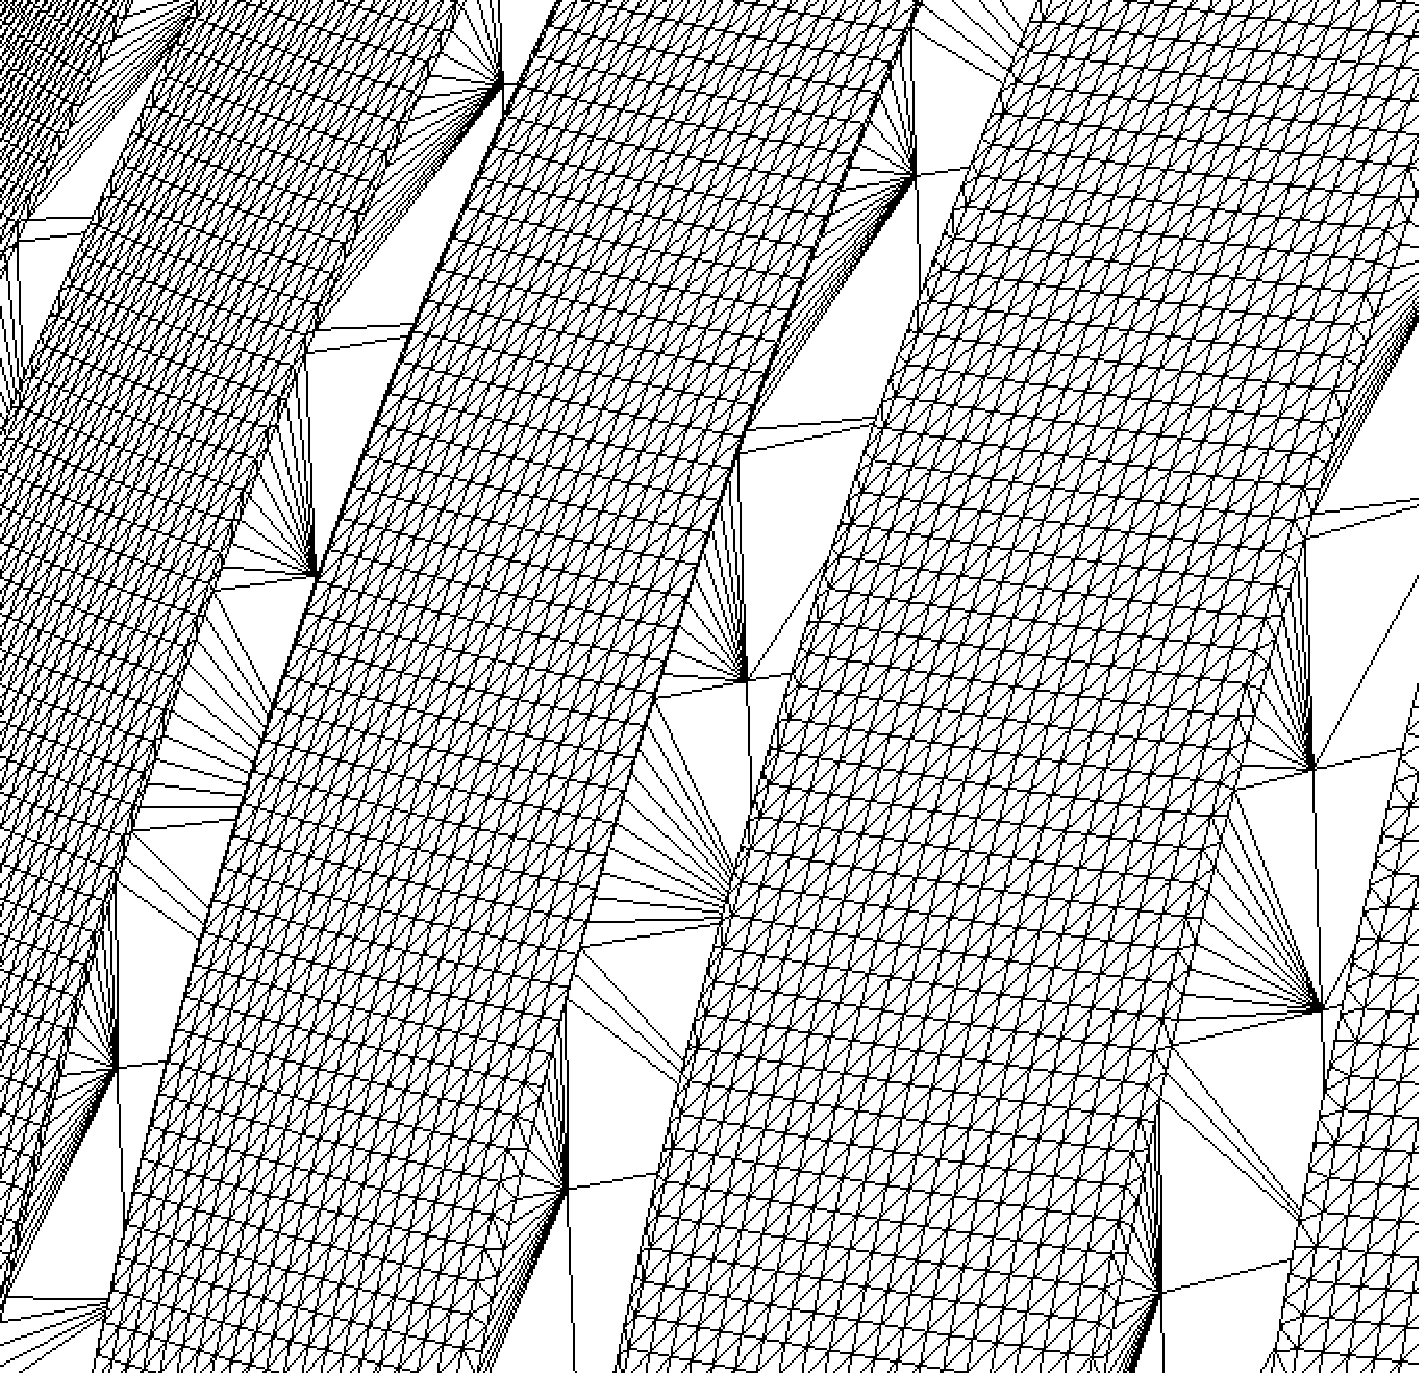
\includegraphics[scale=0.1]{ds_hv.png}
    \caption{Exampels of high valence regions in test and analysis models.}
\end{figure}

To begin, a test mesh was manually generated in MOAB with an artificial high-valence region. This mesh is a modified cube centered on the origin in which the typical two-triangle faceting has been replaced by more complex planar surfce of triangles including an offset interior high-valence region within the face (please see figure below as a reference). The high-valence region was generated by inserting vertices along the diagonal of the interior box and connecting them to the opposing corners of the box. This effectively creates two adjacent high-valence regions, but this was necessary in order to maintain a watertight connectivity in the surface. This construction was designed such that the valence of the corner vertices in the interior region could be controled as well as the size of the interior region relative to the size of the entire face. Tests were then peformed on this model in order to characterize the performance impediment induced as well as its cause.

%TEST MODEL IMAGE HERE

A simple ray fire test program was used to construct ray tracing acceleration structures and conduct ray queries in DAGMC in the same way it would during particle transport. Information on this test program can be found in the appendix of this work. This program was used to fire rays with random direction from the origin of the test model while limiting the scope of the rays such that they should always find intersections on the modified surface containing the high-valence region. Many tests were done while varying the percentage of the surfce covered by the high-valence region as well as the valence of the region. Results using the current state of DAGMC can be found below. 

%INITIAL RESULTS OF HV TESTS HERE

Specification of the random number seed is allowed within the program, giving a more direct comparison of performance with the gaurantee that each test is firing the exact same set of rays.






\bibliographystyle{acm}
\bibliography{refs}


\section{Appendix A: Code used to collect data}
\begin{itemize}
\item ray\_fire\_test program
\end{itemize}

\end{document}
